\hypertarget{la-photographie-en-voyage-un-muxe9tier}{%
\section{La photographie en voyage, un métier
?}\label{la-photographie-en-voyage-un-muxe9tier}}

\emph{Mardi 01 mai 2018}

A l'approche du voyage, nous avons acheté un appareil photo. Un Canon
PowerShot G7X Mark II, vivement recommandé par Pierre.

\begin{figure}
\centering
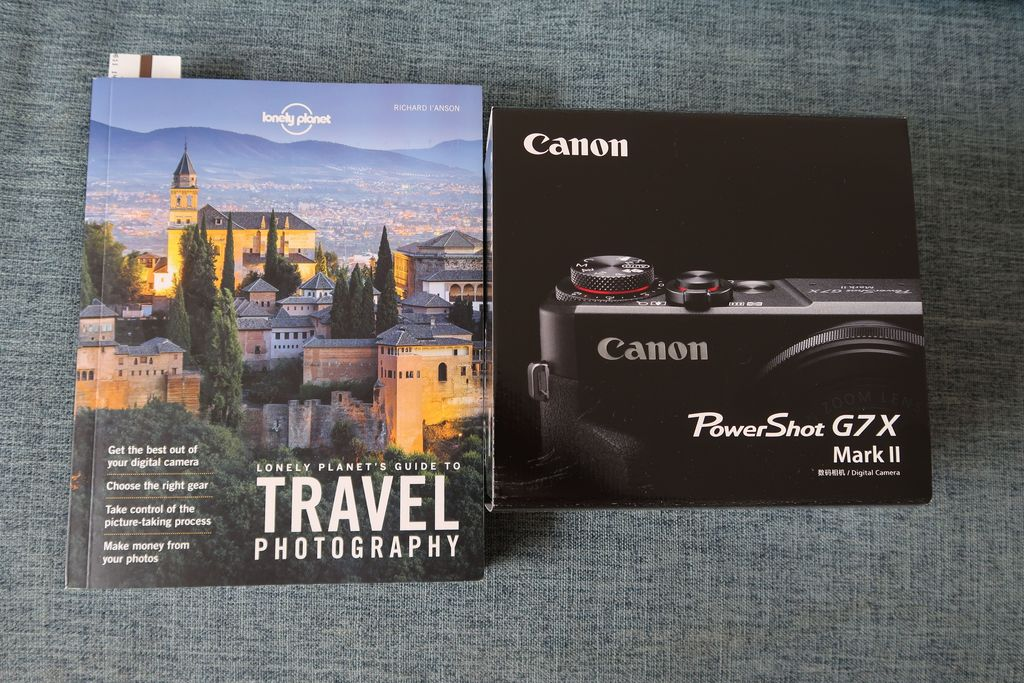
\includegraphics{images/appareil_photo_canon_g7x.JPG}
\caption{La boîte de l'appareil et le livre prêté par Ruocong pour
commencer à appréhender la thématique.}
\end{figure}

L'idée que je m'étais faite est que lorsqu'on est équipé d'un bon
appareil, on fait facilement des bonnes photos. Après quelques semaines
de pratique, je me rends bien compte que ce n'est que la partie émergée
de l'iceberg. On ne devient pas photographe en un jour.

Qu'à celà ne tienne, vous trouverez ci-dessous quelques exemples de
photos prises durant les dernières semaines avec ce bel appareil photo.
Ceci me permet également de tester l'intégration d'une gallerie photo
cliquable dans les articles de blog.

\emph{Florian}

\hypertarget{commentaires}{%
\subsection{Commentaires}\label{commentaires}}

\begin{itemize}
\item
  Thibaud, \emph{2018-05-02 16h40}

  Ça a l'air de bien fonctionner mais peut-être que tu auras envie de
  modifier ton CSS pour centrer les photos et les espacer légèrement :D
  Tu pourrais faire un article sur le CSS ensuite :)
\item
  Florian LB, \emph{2018-05-04 08h37}

  Salut Thibaud ! Déjà, merci pour le commentaire. Bravo, tu es le
  premier ! Le CSS, c'est un sujet sensible, mais j'ai demandé à une
  experte de nous prêter main forte pour améliorer ça. L'idée de faire
  un article sur "comment ce blog est fait" me trotte dans la tête, mais
  je vais sans doute attendre encore pas mal de temps avant de l'écrire.
  A bientôt !
\item
  ZRC, \emph{2018-05-03 08h54}

  Tu trouveras peut-être que la photographie, c'est comme l'optimisation
  : quand on optimise dans un ensemble limité de solutions, l'optimum
  est facile à atteindre, mais quand on passe dans un ensemble plus
  vaste et plus proche des optima globaux (un meilleur appareil photo),
  le problème est plus difficile... C'est un équilibre à améliorer entre
  qualité d'approximation et performance d'estimation, quoi.
\item
  Florian LB, \emph{2018-05-04 08h43}

  Salut ZRC. Tu inaugures avec brio les commentaires à base d'analogies
  mathématiques ! Je commence à voir la photographie d'un autre œil en
  tout cas. Maintenant, à l'attaque de ce nouvel espace...
\item
  Michael, \emph{2018-05-29 21h59}

  \href{https://uploads.disquscdn.com/images/d3d52c79db3c778c55746cf8982dd515cea75ba04db4e5912de5a2f20df6195c.png}{https://uploads.disquscdn.c...}
\item
  Florian LB, \emph{2018-06-01 08h55}

  Haha. On attend des commentaires "photos" de ta part sous chaque
  article maintenant ! :-)
\end{itemize}

